\documentclass{article}
\usepackage[utf8]{inputenc}  
\usepackage[T1]{fontenc}     
\usepackage{amsmath}
\usepackage{hyperref}
\usepackage{listings}
\usepackage{graphicx}

\title{Wykład 1: Rachunek macierzowy}
\author{opracowanie: Jacek Tyszkiewicz}
\date{10.03.2025r.}

\begin{document}

\maketitle

\section{Czy biblioteka numpy jest wydajna?}

Biblioteka \textbf{NumPy} jest napisana głównie w następujących językach programowania:

\begin{itemize}
    \item \textbf{Python} – dla warstwy wysokopoziomowej i interfejsu użytkownika.
    \item \textbf{C} – dla wydajnych operacji numerycznych na tablicach.
    \item \textbf{Fortran} – w niektórych modułach, np. do obsługi funkcji algebraicznych.
\end{itemize}

Dzięki temu NumPy łączy łatwość użycia Pythona z wydajnością języków niskopoziomowych, co czyni go bardzo efektywnym narzędziem do obliczeń numerycznych.
\section{Czemu Rank-1 update jest wydajne?}
Runkt-1 update jest wydajne z tego względu, że przesyłamy dwa wektory 1xn, następnie tworzymy macierz nxn. Przesyłanie danych jest wolne, a utworzenie macierzy pozwala zoptymalizować ten przesył.
\section{Jak zrobić iloczyn skalarny dwóch wektorów?}
Iloczyn skalarny dwóch wektorów:

\[
\begin{bmatrix} -1 & 0 & 2 \end{bmatrix} 
\begin{bmatrix} -1 \\ 2 \\ 1 \end{bmatrix} 
= (-1) \cdot (-1) + 0 \cdot 2 + 2 \cdot 1 = 3
\]
\newpage
\section{Omów dekompozycje macierzy w celu jej wymnożenia}
Mnożenie dwóch macierzy jako złożenie mnożenia wielu wektorów:

\[
\begin{bmatrix} 
3 & -1 & 2 \\ 
1 & 0 & -2 \\ 
-2 & 1 & 3 \\ 
0 & -1 & -3 
\end{bmatrix} 
\begin{bmatrix} 
1 & 0 \\ 
2 & -1 \\ 
-3 & 3 
\end{bmatrix}
\]

Rozkładając mnożenie na poszczególne iloczyny wektorowe, otrzymujemy:

\[
\begin{bmatrix} 
\begin{bmatrix} 3 & -1 & 2 \end{bmatrix} \begin{bmatrix} 1 \\ 2 \\ -3 \end{bmatrix} & 
\begin{bmatrix} 3 & -1 & 2 \end{bmatrix} \begin{bmatrix} 0 \\ -1 \\ 3 \end{bmatrix} \\[10pt]

\begin{bmatrix} 1 & 0 & -2 \end{bmatrix} \begin{bmatrix} 1 \\ 2 \\ -3 \end{bmatrix} & 
\begin{bmatrix} 1 & 0 & -2 \end{bmatrix} \begin{bmatrix} 0 \\ -1 \\ 3 \end{bmatrix} \\[10pt]

\begin{bmatrix} -2 & 1 & 3 \end{bmatrix} \begin{bmatrix} 1 \\ 2 \\ -3 \end{bmatrix} & 
\begin{bmatrix} -2 & 1 & 3 \end{bmatrix} \begin{bmatrix} 0 \\ -1 \\ 3 \end{bmatrix} \\[10pt]

\begin{bmatrix} 0 & -1 & -3 \end{bmatrix} \begin{bmatrix} 1 \\ 2 \\ -3 \end{bmatrix} & 
\begin{bmatrix} 0 & -1 & -3 \end{bmatrix} \begin{bmatrix} 0 \\ -1 \\ 3 \end{bmatrix}
\end{bmatrix}
\]
\section{Mnożenie macierzy jako SUMA rank-1 updates}

Mnożenie dwóch macierzy:

\[
\begin{bmatrix} 
3 & -1 & 2 \\ 
1 & 0 & -2 \\ 
-2 & 1 & 3 \\ 
0 & -1 & -3 
\end{bmatrix} 
\begin{bmatrix} 
1 & 0 \\ 
2 & -1 \\ 
-3 & 3 
\end{bmatrix}
\]

Rozkład na sumę iloczynów wektorowych:

\[
\begin{bmatrix} 
3 \\ 1 \\ -2 \\ 0 
\end{bmatrix} 
\begin{bmatrix} 1 & 0 \end{bmatrix}
+
\begin{bmatrix} 
-1 \\ 0 \\ 1 \\ -1 
\end{bmatrix} 
\begin{bmatrix} 2 & -1 \end{bmatrix}
+
\begin{bmatrix} 
2 \\ -2 \\ 3 \\ -3 
\end{bmatrix} 
\begin{bmatrix} -3 & 3 \end{bmatrix}
\]

Obliczenia elementów macierzy wynikowej:

\[
\begin{bmatrix} 
3 \cdot 1 & 3 \cdot 0 \\ 
1 \cdot 1 & 1 \cdot 0 \\ 
(-2) \cdot 1 & (-2) \cdot 0 \\ 
0 \cdot 1 & 0 \cdot 0 
\end{bmatrix}
+
\begin{bmatrix} 
(-1) \cdot 2 & (-1) \cdot (-1) \\ 
0 \cdot 2 & 0 \cdot (-1) \\ 
1 \cdot 2 & 1 \cdot (-1) \\ 
(-1) \cdot 2 & (-1) \cdot (-1) 
\end{bmatrix}
+
\begin{bmatrix} 
2 \cdot (-3) & 2 \cdot 3 \\ 
(-2) \cdot (-3) & (-2) \cdot 3 \\ 
3 \cdot (-3) & 3 \cdot 3 \\ 
(-3) \cdot (-3) & (-3) \cdot 3 
\end{bmatrix}
\]
\section{Tradycyjna implementacja mnożenia macierzy}
 Implementacja mnożenia macierzy w języku C:

\begin{lstlisting}[language=C]
int mm()
{
    int i, j, k;
    double sum = 0;

    for (i = 0; i < SIZE; i++) { // rows in multiply
        for (j = 0; j < SIZE; j++) { // columns in multiply
            for (k = 0; k < SIZE; k++) { // columns in first and rows in second
                sum = sum + first[i][k] * second[k][j];
            }
            multiply[i][j] = sum;
            sum = 0;
        }
    }
    return 0;
}
\end{lstlisting}
\section{Szybka implementacja mnożenia macierzy: Zarys idei}

Transponujemy macierz \( B \), i rozwijamy pętle mnożenia. Teraz, wartości z macierzy \( A \) jak i wartości z \( B \) przesyłane są z pamięci RAM do cache’a procesora blokami i mnożenie wykonuje się na całym bloku naraz. kompilatory robią to automatycznie.
\begin{figure}[h]
    \centering
    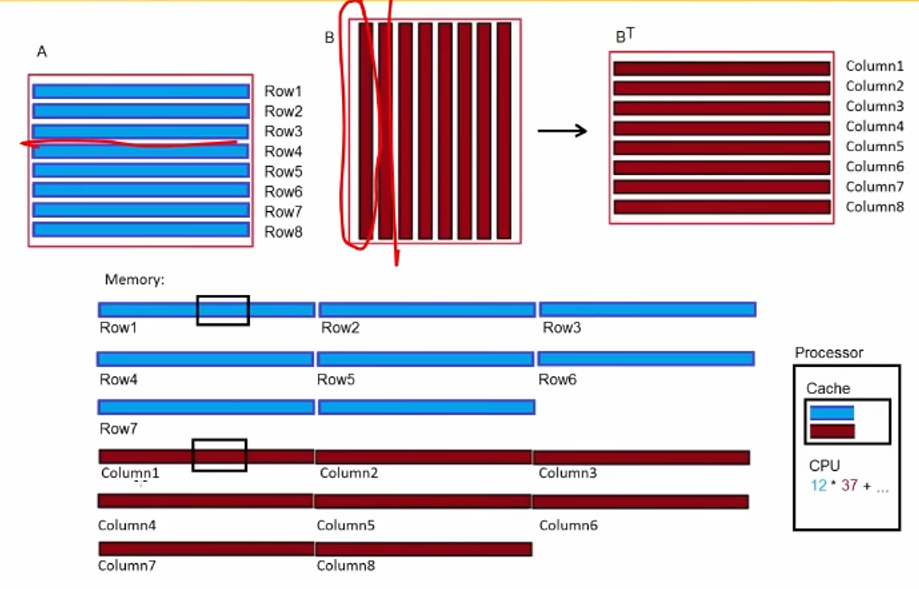
\includegraphics[scale=0.5]{ob1.png}
    \caption{Schemat optymalizacji mnożenia macierzy}
    \label{fig:matrix_mult}
\end{figure}


\section{Blokowe mnożenie macierzy}
Rozważmy mnożenie macierzy w formie blokowej:

\[
\begin{bmatrix}
0 & 0 & 0 & 1 \\
0 & 1 & 0 & 0 \\
0 & 0 & 1 & 0 \\
1 & 0 & 0 & 0
\end{bmatrix}
\begin{bmatrix}
1 & 2 & 3 & 4 \\
5 & 6 & 7 & 8 \\
9 & 10 & 11 & 12 \\
13 & 14 & 15 & 16
\end{bmatrix}
=
\]

Rozdzielamy macierze na bloki:
\begin{figure}[h]
    \centering
    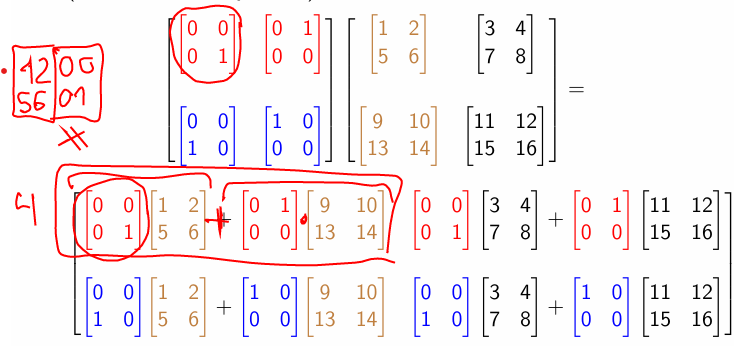
\includegraphics[scale=0.7]{zdj2.png}
    \caption{mnożenie macierzy}
    \label{fig:matrix_mult}
\end{figure}
\begin{figure}[h]
    \centering
    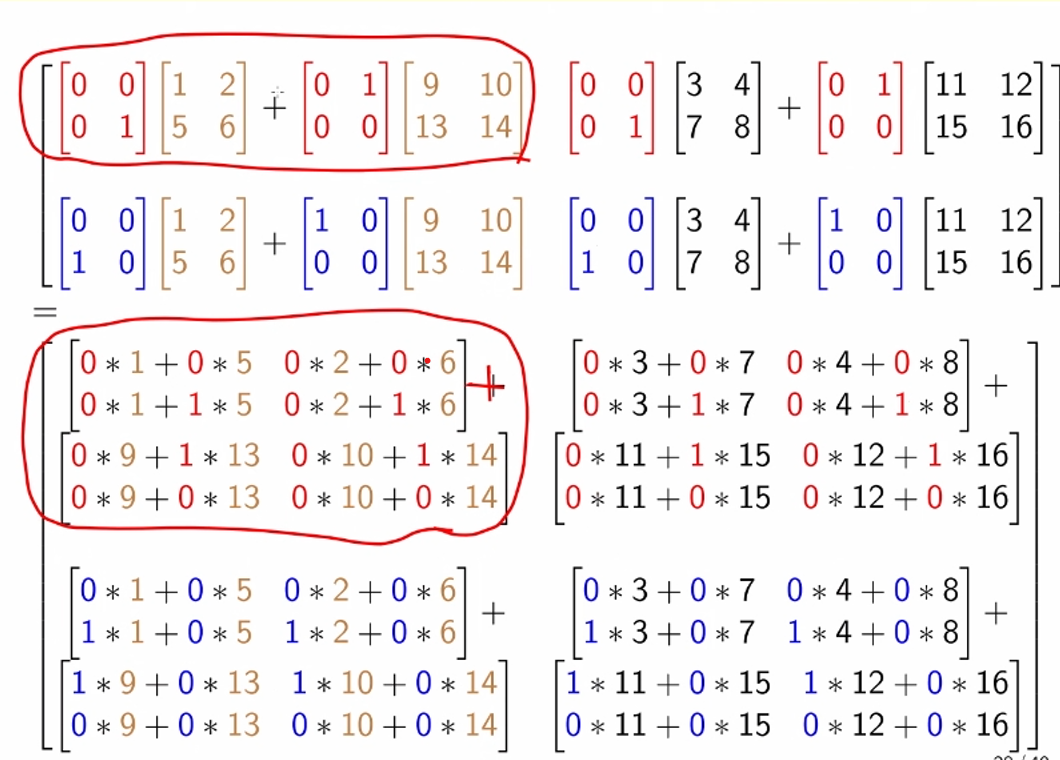
\includegraphics[scale=0.5]{zdj3.png}
    \caption{mnożenie macierzy}
    \label{fig:matrix_mult}
\end{figure}
\newpage
\section{Algorytm Strassena}
Algorytm Strassena to metoda rekursywnego mnożenia macierzy, która redukuje liczbę mnożeń skalarnych z \( O(n^3) \) do około \( O(n^{2.81}) \). Jest to szczególnie przydatne w obliczeniach na dużych macierzach.\\
\\
Rozważmy dwie macierze \( A \) i \( B \), podzielone na \textbf{cztery podmacierze}:

\[
A =
\begin{bmatrix}
A_{11} & A_{12} \\
A_{21} & A_{22}
\end{bmatrix}, 
\quad
B =
\begin{bmatrix}
B_{11} & B_{12} \\
B_{21} & B_{22}
\end{bmatrix}
\]

Zamiast wykonywać 8 blokowych mnożeń, algorytm Strassena definiuje **7 specjalnych iloczynów pośrednich**.\\
\\
\textbf{Siedem iloczynów pośrednich Strassena:}

\[
P_1 = (A_{11} + A_{22})(B_{11} + B_{22})
\]

\[
P_2 = (A_{21} + A_{22}) B_{11}
\]

\[
P_3 = A_{11} (B_{12} - B_{22})
\]

\[
P_4 = A_{22} (B_{21} - B_{11})
\]

\[
P_5 = (A_{11} + A_{12}) B_{22}
\]

\[
P_6 = (A_{21} - A_{11}) (B_{11} + B_{12})
\]

\[
P_7 = (A_{12} - A_{22}) (B_{21} + B_{22})
\]

\textbf{Obliczamy macierz wynikową:}


\[
C =
\begin{bmatrix}
C_{11} & C_{12} \\
C_{21} & C_{22}
\end{bmatrix}
\]

Gdzie:

\[
C_{11} = P_1 + P_4 - P_5 + P_7
\]

\[
C_{12} = P_3 + P_5
\]

\[
C_{21} = P_2 + P_4
\]

\[
C_{22} = P_1 - P_2 + P_3 + P_6
\]

\section{Klasyczny algorytm mnożenia macierzy (Binét) – Omówienie}
Klasyczna metoda mnożenia macierzy, znana również jako \textbf{algorytm Binéta}, polega na standardowej regule mnożenia blokowego macierzy, gdzie każdy element wyniku jest sumą iloczynów odpowiednich wierszy i kolumn.\\
\\
Dla dwóch macierzy \( A \) i \( B \) podzielonych na \textbf{podmacierze}:

\[
A =
\begin{bmatrix}
A_{11} & A_{12} \\
A_{21} & A_{22}
\end{bmatrix}
\quad \text{oraz} \quad
B =
\begin{bmatrix}
B_{11} & B_{12} \\
B_{21} & B_{22}
\end{bmatrix}
\]

macierz wynikowa \( C \) obliczana jest jako:

\[
C =
\begin{bmatrix}
C_{11} & C_{12} \\
C_{21} & C_{22}
\end{bmatrix}
\]

Gdzie bloki \( C_{ij} \) są obliczane według klasycznej reguły mnożenia macierzy:

\[
C_{11} = A_{11} B_{11} + A_{12} B_{21}
\]

\[
C_{12} = A_{11} B_{12} + A_{12} B_{22}
\]

\[
C_{21} = A_{21} B_{11} + A_{22} B_{21}
\]

\[
C_{22} = A_{21} B_{12} + A_{22} B_{22}
\]

\section{Porównanie metod mnożenia macierzy}

\begin{table}[h]
    \centering
    \renewcommand{\arraystretch}{1.5} % Zwiększenie odstępów w tabeli
    \begin{tabular}{|l|c|c|c|}
        \hline
        \textbf{Metoda} & \textbf{Liczba mnożeń} & \textbf{Liczba dodawań} & \textbf{Złożoność} \\
        \hline
        Klasyczny (Binét) & 8 & 4 & \( O(n^3) \) \\
        \hline
        Strassen & 7 & 18 & \( O(n^{2.81}) \) \\
        \hline
    \end{tabular}
    \caption{Porównanie klasycznego algorytmu mnożenia macierzy z metodą Strassena}
    \label{tab:porownanie}
\end{table}
\end{document}
